\chapter{Diseño y Arquitectura}\label{cap:arquitectura}

\section{Arquitectura}
\begin{figure}
	\centering
	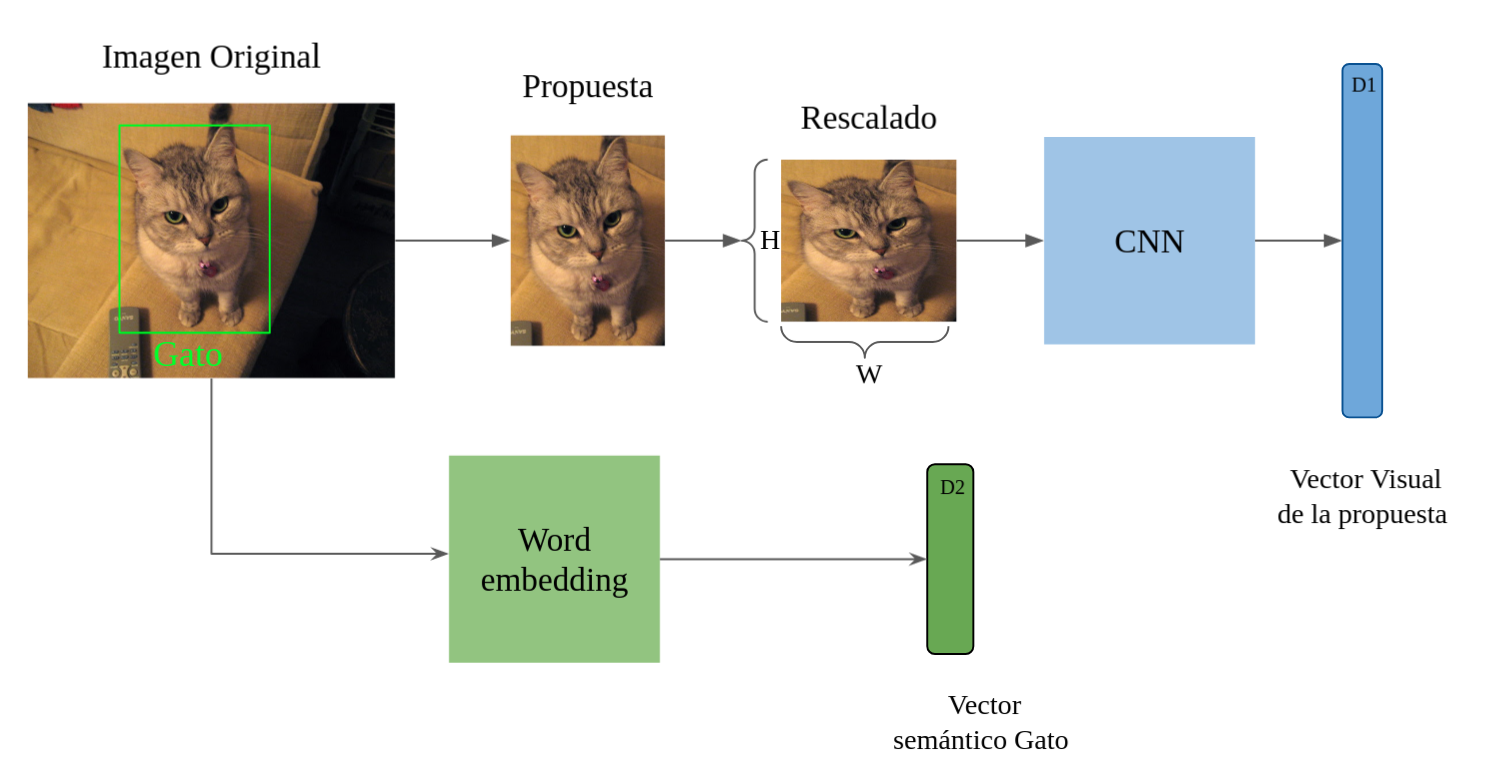
\includegraphics[width=0.9\textwidth]{img/arquitectura.png}
	\caption{Arquitectura propuesta y la dimensión de cada paso.}
	\label{fig:arqutectura}
\end{figure}

Como ya mencionamos anteriormente decidimos basarnos en el modelo propuesto por Ankan Bansal \cite{bansal2018zero}. Su arquitectura propuesta se puede dividir en las siguientes etapas.
\begin{itemize}
	\item \textbf{Pre-procesamiento:} Por cada imagen de entrenamiento, se extrae por cada cuadro delimitador una característica profunda utilizando una red neuronal convolucional y se asocia con la el vector semantico a la clase que corresponde dicho cuadro. Esta etapa nos genera como salida dos listas $X = [\phi(b_0),...,\phi(b_k) \mid \phi(b_i) \in \mathbb{R}^{D_1}]$ $W = [w_0,...,w_k \mid w_i \in \mathbb{R}^{D_2}]$
	\item \textbf{Entrenamiento:} Utilizamos el espacio de incrustación común (${R}^{D_2}$) para calcular una medida de similitud entre las proyecciones  $\phi(b_i)$ y las words embedding  $w_i$. Luego se entrena la proyección usando una pérdida de margen máximo que impone la restricción de que el puntaje de similitud de un cuadro delimitador con su clase verdadera debe ser más alto que el de otras clases. Para esto se utiliza una función de perdida definida como: \[\mathcal{L}(\psi_i, w_i) = \sum_{j \in \mathcal{S}, j\neq i} max(0, m - S_{ii} + S_{ij})\] $m$ es el margen máximo, y $S_{ij}$ es la similitud entre la proyección $i$-$esima$ y la incrustación $j$-$esima$.  También se agrega una función de pérdida de reconstrucción como se hace en \cite{kodirov2017semantic}. Se utilizan las características del cuadro delimitado proyectada para reconstruir las características profundas originales y calcular la pérdida de reconstrucción como la distancia $L2$  entre la característica reconstruida y la característica profunda original. \[\mathcal{L}_r = \Vert{\phi(b_i) - \psi_iW_p^T}\Vert^2 \] Luego definimos $\lambda$ como un coeficiente de ponderación que controla la importancia del primer y segundo término, que corresponden a las pérdidas de proyección y reconstrucción, respectivamente. Por lo cual la función de perdida total es: \[\mathcal{L}_t = \lambda \mathcal{L} + (1-\lambda) \mathcal{L}_r \]
	\item \textbf{Evaluación:} Por cada imagen que no se utilizo en entrenamiento, se genera un conjunto de propuestas de cuadros delimitadores. Luego, se eliminan todos lo que no tienen un puntaje de confianza mayor a un umbral. Para cada cuadro se computa la característica profunda $\phi(b_i)$ y utilizando la matriz $W_p$, para predecir las característica semántica. Por ultimo, se calcula la similitud con todas las características semántica, asignando al nuevo cuadro delimitador la que tenga mayor puntaje.
\end{itemize}
Es común que en la detección de objetos incluyan una clase de fondo para aprender un detector robusto que pueda discriminar eficazmente entre objetos de primer plano y objetos de fondo. En ZSD, esto no es un problema trivial, ya que no sabemos si un cuadro de fondo incluye elementos de fondo como cielo, tierra, bosque, etc. o una instancia de una clase de objeto invisible. En muchos trabajamos se proponen distintas técnicas para abordar este problema, pero no presentan mejoras en evaluaciones cuantitativas. Es por esto que no se incluye una arquitectura que discrimine cuadros de fondos.

Las propuestas de cuadro delimitadores son claves a la hora de evaluar un modelo, ya que una gran cantidad de ellas puede generar ruido y por el otro extremo se puede ignorar una gran cantidad de objetos.  Muchas arquitecturas incluyen una red de propuestas regionales, RPN por sus siglas en ingles. De esta manera entrenan un modelo completo que también aprende a generar propuestas. Por lo que se pudo investigar, en nuestro caso resulta mas conveniente utilizar un modelo pre-entrenado como Edge-Boxes o Selective search.

\section{Conjuntos de datos}
COCO es un conjunto de datos de detección, segmentación y subtítulos de objetos a gran escala. COCO tiene varias características: Segmentación de objetos,  Reconocimiento en contexto,  Segmentación de material de superpíxeles, 330 mil imágenes ($>$ 200 mil etiquetadas), 1,5 millones de instancias de objetos y 80 categorías de objetos.

Específicamente, estamos interesados en archivos de anotaciones. La gran cantidad de instancias de objetos y de categorias, resulta en un conjunto ideal para entrenar y evaluar modelos de ZSD. Ademas la mayoría de la imágenes consta de una gran cantidad de objetos que generan un contexto y no de uno solo centralizado, como son por ejemplo las imagenes del conjunto Visual Genome Dataset. Utilizamos las imágenes de entrenamiento del conjunto COCO 2014 e imágenes del conjunto de validación para realizar pruebas.
\\
Como COCO no provee una separación de los datos para evaluar modelos de ZSD, es necesario crear una forma de dividirlos. Notar que resulta de suma importancia dividir las clases, de tal manera que para todo objeto del conjunto prueba se encuentre otro similar en entrenamiento. Ademas, no se puede encontrar ningún objeto de prueba en los datos de entrenamiento. Dicho esto, se propuso una manera de separar las imágenes. COCO también tiene agrupada las clases por ``Clases superiores''
\begin{figure}[H]
	\begin{center}
	\centering
	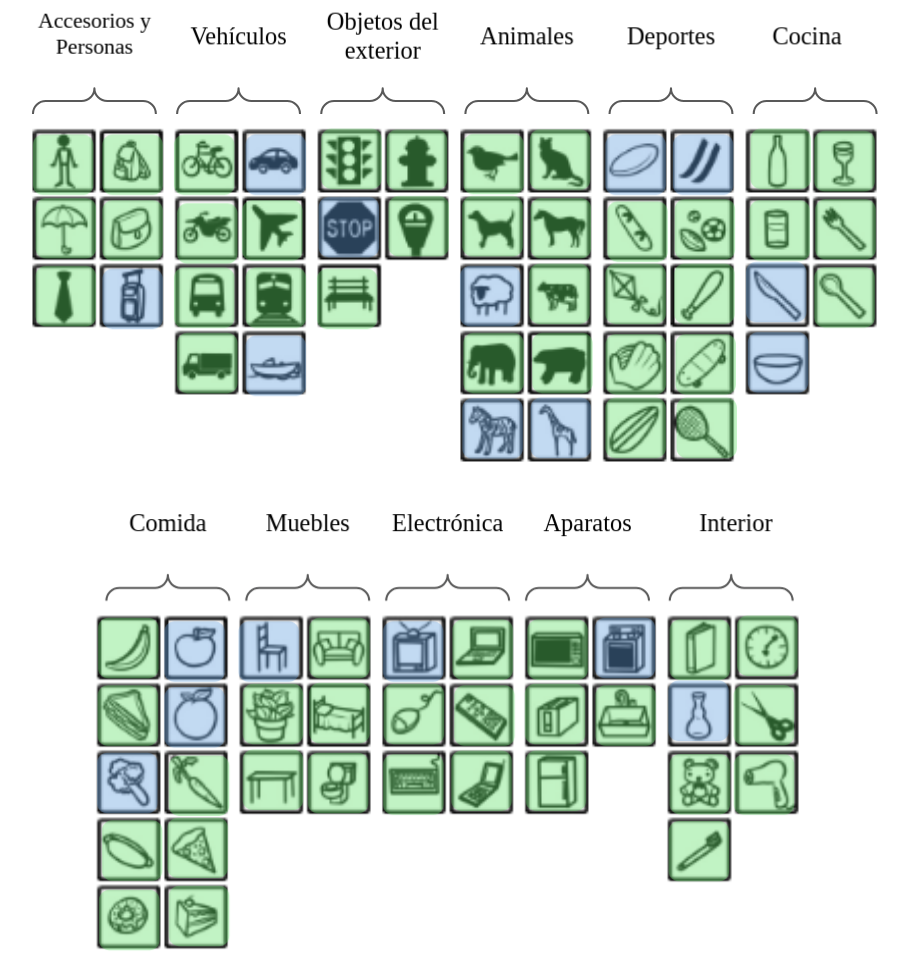
\includegraphics[width=0.9\textwidth]{img/data_set.png}
	\caption{Divisional de las clases para entrenamiento (verde) y pruebas (azul).}
	\label{fig:data_set}
	\end{center}	
\end{figure}
Por cada ``Clase superior'', elegimos de forma aleatoria un 70\% de clases para entrenamiento y un 30\% para pruebas. Es decir 47 y 18 clases respectivamente. En la Figura 3.2 se puede ver como quedan divididas. Por ultimo se eliminaron todas las imágenes de entrenamiento que contengan al menos una instancia de las clases de prueba. Esto resulta en 42564 imágenes con 261258 instancias de entrenamiento y 3008 con 10878 instancias de prueba.

\begin{figure}[H]
	\begin{center}
	\begin{subfigure}{.3\textwidth}
		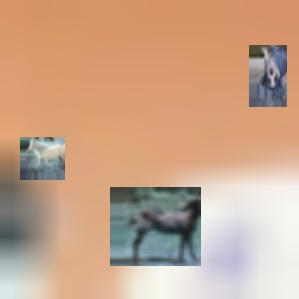
\includegraphics[width=0.85\textwidth]{img/cifar-zsd-test400.jpg}
		\label{fig:ex1}
	\end{subfigure}
	\begin{subfigure}{.3\textwidth}
		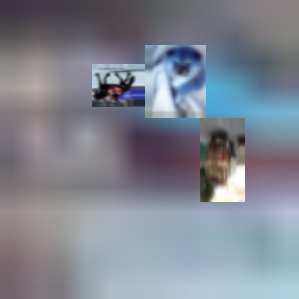
\includegraphics[width=0.85\textwidth]{img/cifar-zsd-test379.jpg}
		\label{fig:ex2}
	\end{subfigure}
	\begin{subfigure}{.3\textwidth}
		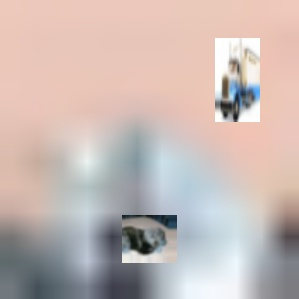
\includegraphics[width=0.85\textwidth]{img/cifar-zsd-test283.jpg}
		\label{fig:ex3}
	\end{subfigure}
	\caption{Ejemplos de imágenes del conjunto de datos CIFAR-ZSD.}
	\label{fig:CIFAR-ZSD}
	\end{center}
\end{figure}

COCO puede resultar pesado lo cual implica mucho tiempo de cómputos, para soluciona esto se creo un conjunto de datos sintéticos basado en CIFAR-100 datasets, el cual denominamos CIFAR-ZSD. Consta de imágenes localizadas, rotadas y re-escalada aleatoriamente con un fondo de otra imagen. Con esto se intenta simular imágenes reales en la cual un objeto puede aparecer con distintos aspectos y escalas. Este conjunto esta divido para que ninguna instancia de prueba  aparezca en el conjunto de entrenamiento.

Aunque resulta muy útil para probar modelos, no es bueno para reportar métricas reales. Pero en combinación con COCO, que si lo es, ambos cooperan para enfrentar el problema de ZSD de una forma mas practica.

\section{Detalles de la implementación}

Primero realizamos un preprocesamiento a todos los datos. Generamos un conjunto de propuestas para todas las imágenes de entrenamiento. Probamos con 2 algoritmos distintos \textbf{Edge Boxes} y \textbf{Selective Search}, mas adelante se presentan las diferencias entre los dos. Luego por cada propuesta se calcula la intersección sobre unión con todos los cuadros delimitadores verdaderos. Si el IoU $> 0.5$ con algún cuadro verdadero, lo anotamos con la clase de dicho cuadro. Si el IoU $<= 0.2$ para todos los cuadros de verdad, se anota como clase de fondo, con una probabilidad del 0.0001. La clase de fondo en nuestro modelo no es utilizada. Este preprocesamiento aumenta significativamente la canitdad de instancias para entrenamiento. Para COCO se tiene un total de 1.436.835 instancias y 137.204 para CIFAR-ZSD. \\

El siguiente paso es para cada box generar el vector de características visuales y semánticas. Para el primero, se probo con dos CNN, \textbf{VGG16} y \textbf{Inception ResNet V2}. Se defino el tamaño de los cuadros delimitadores de entrada en $224 \times 224$ para VGG16 y $299 \times 299$ en ResNet. El tamaño del vector de salida es de 512 en VGG y 1536 ResNet. Para ambos usamos pesos preentrenado en \textbf{Imagenet}. Esto es una diferencia con Bansal \cite{bansal2018zero}, ya que en este trabajo el modelo se entrena de extremo a extremo, es decir los pesos de la CNN se ajustan en la etapa de entrenamiento.

Para obtener las características semánticas, utilizamos Word2vec con un corpus de Google News (3 mil millones de palabras) entrenado previamente 3 millones de vectores de palabras en inglés de 300 dimensiones.\\

Por ultimo para entrenamiento se creo una red con una sola capa oculta, una capa de entrada del tamaño del vector de características visuales y una de salida de la dimensión de las características semánticas. Se utilizo un optimizador adam, sin ninguna activación, con un taza de aprendizaje de 10e-3 y un tamaño del lote de 64. Para la función de perdida se uso un lambda de 10e-3 y un margen máximo de 1.\\

El codigo esta implementado en Python 3 utilizando Keras con TensorFlow de backend. Por mas detalles se deja el link al codigo.\\\url{https://github.com/agustinhurquiza/Tesis}


